\documentclass{article}

\usepackage[utf8]{inputenc}
\usepackage[norsk]{babel}
\usepackage{amsmath,amsfonts,amssymb,amsthm,mathtools} % Most people will need these for mathematics


\usepackage{minted}             % syntax highligting
\usepackage[dvipsnames]{xcolor} % colors


\usepackage{hyperref}           % linker i dokumentet
\hypersetup{
    colorlinks=true,
    linkcolor=black,
    filecolor=magenta,      
    urlcolor=ForestGreen,
}

\urlstyle{same}
\usepackage{fancyvrb}
\usepackage{float}
\usepackage{booktabs}
\usepackage{csquotes}
\usepackage{enumitem}
\usepackage{tcolorbox}

% \usepackage{pgfplots}

\usepackage{titlesec}
\usepackage{amsmath}
\usepackage{amsthm}
\usepackage{amsfonts}
\usepackage[normalem]{ulem}
\usepackage{amssymb}
\usepackage{multicol}
\usepackage{multirow}
\usepackage{fancyhdr}
\pagestyle{fancy}
\fancyhead{}
\renewcommand{\headrulewidth}{0.1pt}
\fancyhead[C]{Rapport Software Engineering}
\usepackage{pgfplots}
\pgfplotsset{compat=1.10}

\usepackage{tabularx}
\setcounter{secnumdepth}{4}

\titleformat{\paragraph}
{\normalfont\normalsize\bfseries}{\theparagraph}{1em}{}
\titlespacing*{\paragraph}
{0pt}{3.25ex plus 1ex minus .2ex}{1.5ex plus .2ex}
% Formattering av paragrafer indentering og skip
% \setlength{\parindent}{0em}
% \setlength{\parskip}{1em}




\title{Software Engineering Dokumentasjon}
\author{%
	\large
	\textsc{Gruppe 19}\\
	\textsc{Gruppe 193306}
	\normalsize	H{\o}gskolen i {\O}stfold \\
	\vspace{-5mm}	
}

\begin{document}

%----------------------------------------------------------------------------------------
%	TITLE PAGE
%----------------------------------------------------------------------------------------

\begin{titlepage} % Suppresses headers and footers on the title page

	\centering % Centre everything on the title page
	
	%------------------------------------------------
	%	Top rules
	%------------------------------------------------
	
	\rule{\textwidth}{1pt} % Thick horizontal rule
	
	\vspace{2pt}\vspace{-\baselineskip} % Whitespace between rules
	
	\rule{\textwidth}{0.4pt} % Thin horizontal rule
	
	\vspace{0.1\textheight} % Whitespace between the top rules and title
	
	%------------------------------------------------
	%	Title
	%------------------------------------------------
	
	{\Huge \uppercase{\textbf{Gruppeprosjekt}} \\[0.5\baselineskip] }

	\textcolor{Red}{ % Red font color
		{\Large \textbf{Software Engineering}} \\[0.3\baselineskip] % Title line 1
	}
	
	\uppercase{Høst 2020}
	
	\vspace{0.3em} % Whitespace between the title and short horizontal rule
	
	\rule{0.3\textwidth}{0.4pt} % Short horizontal rule under the title
	
	\vspace{0.1\textheight} % Whitespace between the thin horizontal rule and the author name
	
	%------------------------------------------------
	%	Author
	%------------------------------------------------

	\vspace{0.6em}
	
	{\large \textsc{
	    Fabian Berget Lindblad \\[0.1em] 
	    Kacper Rafal Sliwa \\[0.1em] 
	    Rikke Hedelund Hansen \\[0.2em] 
	    Aleksander Lengard
	    }
    } % Author name
    
	\rule{0.3\textwidth}{0.4pt}
	\vspace{0.3em}
	
    \textcolor{Red}{
        \uppercase{\textbf{Gruppe 19}}
	}
	
	\vfill % Whitespace between the author name and publisher
	
	%------------------------------------------------
	%	Publisher
	%------------------------------------------------
	
% 	{\large\textcolor{Red}{\plogo}}\\[0.5\baselineskip] % Publisher logo

	{\large\textsc{Høgskolen i Østfold\\	
		Avdeling for informasjonsteknologi}} % Publisher
	
	\vspace{0.1\textheight} % Whitespace under the publisher text
	
	%------------------------------------------------
	%	Bottom rules
	%------------------------------------------------
	
	\rule{\textwidth}{0.4pt} % Thin horizontal rule
	
	\vspace{2pt}\vspace{-\baselineskip} % Whitespace between rules
	
	\rule{\textwidth}{1pt} % Thick horizontal rule

\end{titlepage}

% \maketitle
\thispagestyle{empty} % fjerner side tall fra forsiden

\newpage
% starter side telling etter forsiden
\setcounter{page}{1}
\tableofcontents
\newpage

% Endrer indentering på paragrafer
\setlength{\parindent}{0em}
\setlength{\parskip}{0,7em}

\section{Innledning}
% \textbf{FOR HELE OPPGAVEN:\\
% IKKE AKADEMISK RAPPORT, MEN FOR EN KUNDE OG UTVIKLINGSPARTNER. \\
% BESKRIVER PROBLEMSTILLINGEN OG LØSNINGEN\\
% FORSTÅELIG FOR IKKE TEKNISKE PERSONER MED DOMENEKUNNSKAP \\
% FLYTEN ER HENSIKTMESSIG FOR Å PRESENTERE PROSJEKT PÅ EN FORSTÅELIG MÅTE\\
% VÆRE ET OMFANG OG HA ET INNHOLD SOM GJØR DET ER TYDELIG AT DEN ER GRUNNLAGT FOR PROTOTYPEN}

I faget Software Engineering og Testing har gruppen fått i oppgave å lage produktdokumentasjon for en tjeneste en oppstartsbedrift ønsker å utvikle. Vi skal skape kjernesystemet i denne tjenesten, og avdekke hvilke funksjoner og egenskaper som må være med for å imøtekomme kundens ønske. I tillegg skal det lages en prototype, et «minste brukbare produkt» som viser hvordan systemet er tenkt brukt.  

\subsection{Gruppemedlemmer}
\begin{multicols}{2}
\begin{itemize}
    \item[] Fabian Berget Lindblad \newline
    \textit{Informatikk, 2. året. }\newline
    \href{matilto:fabian.b.lindblad@hiof.no}{fabian.b.lindblad@hiof.no}
    
    \item[] Kacper Rafal Sliwa \newline
    \textit{Informasjonssystemer, 2. året. }\newline
    \href{mailto:kacper.r.sliwa@hiof.no}{kacper.r.sliwa@hiof.no}

    \item[] Rikke Hedelund Hansen \newline
    \textit{Informatikk, 2. året. }\newline
    \href{mailto:rikke.h.hansen@hiof.no}{rikke.h.hansen@hiof.no}
    
    \item[] Aleksander Lengard \newline
    \textit{Informatikk, 2. året. }\newline
    \href{mailto:aleksander.lengard@hiof.no}{aleksander.lengard@hiof.no}
\end{itemize}
\end{multicols}



\section{Introduksjon}

\subsection{Bakgrunn}
I ett samfunn hvor fler og fler bruker bil som transportmiddel, er det ett stadig økende problem i storbyer en mangel på parkeringsplasser. Det er flere som bor i utkanten og jobber i sentrum og gjerne bruker bilen til og fra jobb. Dette har skapt en stor etterspørsel etter parkering, noe som ikke prioriteres i moderne byutvikling. De plassene som allerede er tilgjengelig er gjerne dyre og ikke alltid tilgjengelig der du trenger dem. Men det finnes også de som eier parkeringsplasser eller områder som det kan være mulig for folk å parkere. Noen har parkeringsplass i forbindelse med boligen de eier, men kanskje ikke har bil. Eller bruker sin egen bil til jobb, og dermed er parkeringsplassen ledig i normal arbeidstid.

Det er vanskelig for privatpersoner å ha en oversikt og håndtere dette på egenhånd. Så det er dermed et ønske om å utvikle en tjeneste hvor brukere, kan leie tilgjengelige parkeringsplasser i perioder. Og leie ut sin egn plass når de ikke trenger den selv.

% I en samfunn hvor flere og flere mennesker har bil, så har det blitt laget flere parkeringsplasser i sentrum. Disse parkeringsplassene er dyre å booke, dermed er det mer ettertraktet å leie parkeringsplasser for en hvis tidsperiode. For vanlige privatpersoner og små firmaer er det vanskelig å håndtere den digitale infrastrukturen som er rundt disse parkeringsplasser som hvor man finner parkeringsplass, hvor man kan legge de til leie og lignende.

% Det er da et ønske å utvikle et felles system hvor de kan håndtere mest mulig av det som angår brukere.I tjenesten skal noen aktører kunne registrere tilgjengelige plasser som kan leies ut, mens sluttbrukere kan se, reservere og betale for parkeringsplassen i den tiden de trenger det.


\subsection{Problemstilling}
Tjenesten skal ha funksjoner som på en enkel måte lar brukere leie andre sine parkeringsplasser. Og leie ut sin egen om de ønsker det. Betaling for leien skal skje igjennom tjenesten.

Det skal også være mulig for brukeren å se en oversikt over de plassene man selv leier ut. Og plasser som tidligere har vært leid.

Ett ønske er at tjenesten skal være tilgjengelig på pc, nettbrett og telefon. Slik at man lett kan bruke tjenesten når man ønsker det.

% Tjenesten skal ha funksjoner som gjør det mulig å leie parkeringsplasser og legge ut parkeringsplasser for andre å leie. Den skal også være brukervennlig slik at de fleste forstår tjenesten. 

%  Den skal også være mulig å se en oversikt over de utleide plassene aktøren har og de leide plassene aktøren leier. 
% Det skal også være mulig å betale for de ulike parkeringsplassene, slik at alt det digitaliserte infrastrukturen er implementert i selve tjenesten. 

% En av problemstillingene vi ønsker er at den skal være mulig å være på både telefon, tablet og datamaskiner, og at den er tilpasset til alle. Og at den ikke bryter noen regler.


\subsection{Mål}

For at tjenesten skal være tilgjengelig på flere plattformer trenger kjernesystemet å være tilgjengelig via internett. Ved å lage en API (\textit{application programming interface}) så kan forskjellig typer brukergrensesnitt kommunisere med systemet på samme måte. Dette uten å måtte tilpasse kjernesystemet til de forskjellige. Det er kjernesystemet som behandler alt av forespørsler, og det er her forretningens logikk håndterer dataflyten til og fra databasen.

\begin{figure}[H]
    \centering
    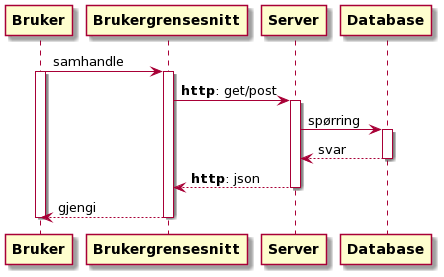
\includegraphics[width=10cm]{bilder/uml/intro_flyt.png}
    \caption{Overordnet oversikt over dataflyt mellom brukergrensesnitt, server og database.}
    \label{fig:lagdeling}
\end{figure}

I denne oppgaven har vi valgt å lage ett forenklet brukergrensesnitt for nettleseren. Men muligheten er mange hvor en slik tjeneste kan passe inn.  Man kan skape mobilapplikasjon eller mulighet for å integrere tjenesten i andre systemer, slik som hotell bookingsider, airbnb eller liknende.

Målet er også å skape brukervennlige funksjoner, som er lette å forstå. Slik at tjenesten skal kunne brukes av voksne i alle aldre, uten spesielt teknisk kunnskap.  Tjenesten skal oppfyller de kravene som raskest gir kunden verdi. I form av en prototype har vi utviklet et «\textit{minste brukbare produkt}» (engelsk: «\textit{minimum viable product (MVP)}»). Som viser kjernefunksjonene i systemet.



For at oppstartsbedriften skal kunne tjene penger på ideen sin. Er det viktig at løsningen vil generer penger, og brukere samtidig. Vi foreslår at brukere som kun leier plass ikke trenger å betale noe for tjenesten. Og for de som ønsker å leie ut, så er de første 6 månedene avgiftsfrie. Etter det vil det påløpe ett gebyr på 20\% av leieinntektene. Dette vil sørge for at brukere som er interessert kan prøve tjenesten kostnadsfritt. Og på den måten skape en brukerbase raskest mulig. Skal du leie ut mer enn 3 plasser, blir du ansett som næringsdrivende. Da vil det bli en løpende månedskostnad på noen hundre kroner.


Videre i denne prosjektdokumentasjonen vil vi beskrive de forskjellige delene av systemet i mer detalj. Og forklare mer om hva og hvordan vi har tenkt at et slik system skal virke. Hvem dens brukere er, vise til tenkte bruker scenarioer, estimere og forklare vår prototype.


% Det er derfor viktig at programvaren har mulighet for å virke både på mobil, gjerne via en applikasjon og i nettleseren. Begge disse plattformene bruker internett for å kommunisere, og vil da være lurt at selve systemet som håndterer alt av databaser og buisness-logikk kan kommuniseres med via en API (\textit{application programming interface}). Dette muliggjør at systemet kan utvides med forskjellige typer brukergrensesnitt i fremtiden. Uten å måtte endre på kjernen i systemet. I denne oppgaven vil vi bruke et forenklet brukergrensesnitt for nettleseren. Men muligheten er mange. Man kan skape mobilapplikasjon eller mulighet for å integrere tjenesten i andre systemer, slik som hotell booking sider, air-bnb eller liknende.
% Målet er også å ha brukervennlige funksjoner, som er lett å forstå. Og at tjenesten oppfyller de kravene vi setter som MVP (\textit{minimum viable product}) som gir kundene verdi.


%  Videre i denne prosjektdokumentasjonen vil vi beskrive de forskjellige delene av systemet i mer detalj. Og forklare mer hva og hvordan vi har tenkt at et slik system skal virke, hvem dens brukere er, vise til tenkte bruker scenarioer, estimere og forklare vår prototype.

\include{Målgruppe}


\section{Krav}
\textit{Kravene skal være beskrevet tydelig, identifiserbar, hensiktsmessig detaljnivå, dekker nødvendige funksjoner i systemet. }

Denne seksjonen forteller om kravene vi finner til systemet, altså krav til innholdet. Det vil si alle funksjoner og funksjonaliteter som blir implementert i systemet. Disse finner vi ved hjelp av brukerhistoriene, user casene og user case diagrammet som vi har laget i forrige seksjon.

%Ut ifra brukerhistoriene, usercase og user case diagrammet har vi kommet fram til kravene for tjenesten. Det vil tilsvare de funksjonene vi vil implementere til systemet.

Vi har definert flere roller i kravene. Disse rollene er bruker, utleier, firma og administrator. Det er for å spesifisere hvilke funksjoner som passer til ulike roller. Utleier og bruker går under det samme i systemet, mens administrator, på den andre siden, er en bruker eller et firma med ekstra rettigheter. 
%I systemet er bruker og utleier det samme og admin er en bruker eller firma med ekstra rettigheter. 
%hva slags funksjoner er tenkt til hvem. em de forskjellige funksjonene er tenkt til.

Firma er en bedriftskunde. De kan bare leie ut plasser, og vil betale en månedlig sum for tjenesten. 
Utleierne er privatpersoner som leier ut parkeringsplassene sine. De vil betale en prosentdel av inntekten etter en viss periode.

Brukerne er privatpersoner som kan leie parkeringsplasser. De vil betale for plassen gjennom tjenesten. 
Administrator er eierene av tjenesten. 
Personene under denne tittelen skal bidra med å holde tjenesten saklig.

\subsection{Funksjonelle krav}
\subsubsection{Opprette bruker}
\label{registere_bruker}
Brukeren/firma/utleieren skal kunne opprette en ny bruker i tjenesten.
\begin{enumerate}[label=(\alph*)]
    \item Brukeren/firma/utleieren skal kunne opprette en bruker i tjenesten med hjelp av epost adresse.
    \item Brukeren/utleieren skal kunne opprette en bruker i tjenesten med hjelp av Facebook konto.
    \item Brukeren/firma/utleieren skal kunne opprette en bruker i tjenesten med hjelp av Google konto.
    \item Firma må oppgi organisasjonsnummer ved opprettelse av bruker.
\end{enumerate}


\subsubsection{Logge inn}
\label{logge_inn}
Brukeren/firma/utleieren skal kunne logge inn i tjenesten.
\begin{enumerate}[label=(\alph*)]
    \item Brukeren/firma/utleieren skal kunne logge inn i tjenesten med hjelp av epost adresse.
    \item Brukeren/utleieren skal kunne logge inn i tjenesten med hjelp av Facebook konto.
    \item Brukeren/firma/utleieren skal kunne logge inn i tjenesten med hjelp av Google konto.
    \item Ved feil brukernavn eller feil passord skal systemet gi beskjed til brukeren at brukernavn eller passord er feil.
    \item Bruker/firma/utleier skal få beskjed om feil, hvis verifiseringen er feil.
    \item Brukeren/firma/utleieren skal kunne gjenopprette konto ved glemt passord.
\end{enumerate}

\subsubsection{Tofaktorisering}
\label{tofaktor}
Tjenesten skal kunne logge seg inn i tjenesten med tofaktorautentisering.
\begin{enumerate}[label=(\alph*)]
    \item Brukeren/firma/utleieren skal kunne ha muligheten å slå på       tofaktorautentisering for å logge inn på kontoen.
    \item Administrator skal kunne ha tofaktorautentisering for å logge inn på kontoen.
    \item Utleieren/firma skal ha tofaktorautentisering for å legge ut en parkeringsplass.
    \item Brukeren/firma/utleieren skal ha tofaktorautentisering for å redigere brukerkonto informasjon om seg selv.
    \item Tofaktorautentisering skal kunnes gjøres med en SMS.
    \item Tofaktorautentisering skal kunne gjøres med en  autorisering applikasjon.
\end{enumerate}

\subsubsection{Legge inn/ redigere parkeringsplass}
\label{Legge_parkering}
Utleieren skal kunne legge til parkeringsplass i tjenesten, slik at den kan bli leid ut.
\begin{enumerate}[label=(\alph*)]
    \item Firma skal kunne legge inn parkeringsplasser inn i tjenesten.
    \item Utleieren skal kunne bestemme prisen på sine parkeringsplasser for ulike tidsrom.
    \item Utleieren skal kunne sette plassen utilgjengelig de dagene utleier bruker plassen selv.
    \item Ved utleie av større område (næring) skal det være mulig å spesifisere antall plasser.
    \item Firma skal kunne bestemme prisen på sine parkeringsplasser for ulike tidsrom.
    \item Utleieren skal kunne redigere informasjonen om sine egne parkeringsplasser.
    \item Firma skal kunne redigere informasjon om sine egne  parkeringsplasser.
    \item Administrator skal kunne redigere informasjon om en parkeringsplass.
\end{enumerate}


\subsubsection{Leie parkeringsplass}
\label{leie_park}
Brukeren skal kunne leie en parkeringsplass i et gitt tidsrom.
\begin{enumerate}[label=(\alph*)]
    \item Brukeren skal kunne få en bekreftelse at parkeringsplassen er kjøpt av brukere for det gitte tidsrommet
    \item Brukeren skal kunne se antall utilgjengelig og tilgjengelig plasser på en lokasjon.
\end{enumerate}


\subsubsection{Søke parkeringsplasser}
\label{søke_park}
Bruker skal kunne søke opp parkeringsplasser.
\begin{enumerate}[label=(\alph*)]
   \item Brukeren skal kunne se tilgjengelige plasser i ønsket område i kart.
\end{enumerate}

\subsubsection{Brukerprofil}
\label{bruker_profil}
Brukeren/firma/utleieren skal kunne ha en brukerprofil.
\begin{enumerate}[label=(\alph*)]
    \item Brukeren skal kunne se oversikt over leide plasser.
    \item Utleieren/firma skal kunne se oversikt over sine egne parkeringsplasser.
    \item Brukeren skal kunne se tidligere leide plasser.
    \item Brukeren/firma/utleieren skal kunne redigere brukerkonto informasjon om seg selv.
    \item Administrator skal kunne se en oversikt over alle brukere.
    \item Administrator skal kunne se en oversikt over alle utleide plasser og hvem som har leid de ut.
    \item Utleieren/firma skal kunne se en oversikt av inntjeninger av parkeringsplass(ene). 
    \item Tjenesten skal vise en oversikt av inntjeninger i form av kakegrafer.
\end{enumerate}



\subsubsection{Betaling}
\label{betaling}
Brukeren skal kunne betale for leie og utleie av parkeringsplasser ved å bruke Vipps/Mastercard.
\begin{enumerate}[label=(\alph*)]
  \item Brukeren skal ha muligheten til   å få en betalingen refundert maks   10 minutter etter et eventuelt feilkjøp.
    \item Det skal være tydelig hva betalingen er så en bruker ikke blir usikker på om betalingen/produktet er feil. 
    \item Brukeren skal ha mulighet til å se alle sine tidligere betalinger.
    \item Brukeren skal kunne avbestille den kjøpte parkeringsplassen og få pengene tilbake, 24 timer før parkeringen starter.
    \item Firma skal kunne betale en fast månedsbeløp for å bruke tjenesten med faktura/avtalegiro.
    \item Utleieren skal kunne betale en prosentvis av leieinntektene etter 6 måneders gratisperiode.
    \item Tjenesten skal kunne ha en konto hvor betalingene til de ulike funksjonene blir overført. 
    \item Utleieren skal kunne få pengene fra utleie av parkeringsplassene sine gjennom tjenesten sin konto.
\end{enumerate}

\subsubsection{Redigering av informasjon}
\label{redigering}
Administrator skal kunne redigere innholdet på siden, slik som "ofte stilte spørsmål" og nyheter

%Notasjon, annotasjon, bemerkning, anmerkning, kommentar, notis?
\subsubsection{Varsler}
\label{merking}
Brukeren skal kunne varsle om en utleier som usaklig/upassende
\begin{enumerate}[label=(\alph*)]
    \item Utleieren skal kunne varsle om en bruker er usaklig/upassende.
    \item Firma skal kunne varsle en bruker som usaklig/upassende
\end{enumerate}

\subsubsection{Fjerne parkeringsplass/bruker/profil}
\label{fjerne}
Utleieren/firma skal kunne fjerne sine egne parkeringsplasser.
\begin{enumerate}[label=(\alph*)]
    \item Administrator skal kunne fjerne en bruker/utleier som er usaklig/upassende.
    \item Administrator skal kunne fjerne parkeringsplasser som er usaklig/upassende.
    \item Brukeren/firma/utleier skal kunne slette sin egen profil.
    
\end{enumerate}

\subsubsection{Verifisering}
\label{verifisering}
Administrator skal kunne verifisere at parkeringsplassen tilhører faktisk utleieren/firma
\begin{enumerate}[label=(\alph*)]
    \item Administrator skal kunne fryse en annonse frem til eierskap av plassen er bekreftet
\end{enumerate}

\subsubsection{Hjelp og Support}
\label{hjelp_support}
Tjenesten skal være enkelt å bruke og lett å få hjelp. Dette gjøres ved at:
\begin{enumerate}[label=(\alph*)]
    \item Brukeren/firma/utleieren skal kunne se kontaktinformasjon til kundestøtte.
    \item Brukeren/firma/utleieren skal kunne se ofte stilte spørsmål som administrasjonen . 

\end{enumerate}

%\subsubsection{Kontakt}
%\textit{Administrator skal kunne kontakte brukere av systemet.}
%\begin{enumerate}[label=(\alph*)]
 %   \item Brukeren skal kunne kontakte admin angående useriøse hendelser.
 %   \item Utleieren/firma skal kunne kontakte admin angående useriøse hendelser.
%\end{enumerate}


\subsection{Ikke-funksjonelle krav}
%\textit{Tjenesten skal utformes i tråd med lovgivingen i GDPR. Alle underleverandører skal også oppfylle kravene til GDPR. }
\subsubsection{Personopplysningsloven}
\label{personvern}
Tjenesten skal tilfredsille krav i personopplysningsloven, som omhandler innsamling og bruk av personopplysninger. Dette gjelder de nasjonale reglene, samt EUs personvernsforordning (GDPR - General Data Protection Regulation). \newline
- \href{https://www.datatilsynet.no/regelverk-og-verktoy/lover-og-regler/}{Datatilsynet}

\subsubsection{Krav om universell utforming}
\label{universell_u}
Tjenesten skal som ett minimum tilfredstille minstekravet, beskrevet i det kommende regelverket for universell utforming av IKT-løsninger, WAD og WCAG 2.1.\newline 
- \href{https://uu.difi.no/}{Digitaliseringsdirektoratet}



\subsubsection{Sikkerhet}
\label{sikkerhet}
Databasen skal sikres mot angrep, ved at det blir tatt backup av databasen.
\begin{enumerate}[label=(\alph*)]
    \item En betaling skal verifiseres i løpet av maks 3 sekunder. 
    \item Kortnummer og lignende skal ikke bli lagret for en bruker og være kryptert under en betaling.
\end{enumerate}

\subsubsection{Tekniske krav}
\label{teknisk_krav}
Applikasjon skal bli programmert i: 
\begin{enumerate}[label=\alph*]
    \item Node.js
    
\end{enumerate}


\subsubsection{Eksterne Avhengigheter}
\label{ekstern_avhengihet}
Tjenesten skal ha forskjellige eksterne avhengigher. Disse avhengighetene er
\begin{enumerate}[label=(\alph*)]
    \item NoSQL Database som gjør at det er lettere å skalere.
    \item Betalingstjeneste som Vipps og Mastercard.
    \item Google Maps.
    \item Innloggingssystem som Facebook og Google.
\end{enumerate}


\subsection{Videre utvikling av tjenesten}
For å utvikle tjenesten ytterligere, kan man legge til et system hvor brukere kan gi tilbakemelding på parkeringsplassen de har leid. Dette kan være i form av stjerner eller liknende som baserer seg på deres erfaring slik som plassens lokasjon, pris, og om den var lett å komme til. Det vil også være mulig å legge inn en kommentar

Som nevnt tidligere i oppgaven, så er det ett bevisst ønske at systemet skal være tilgjengelig med en API. Dette for at senere kan utvikles flere plattformer hvor brukere kan benytte seg av systemet. Dette innebærer mobilapplikasjon, integrering i fysiske maskiner, slik som parkerings automater og liknende.

Det kan legges til en innebygd chattefunksjon mellom bruker og utleier som en del av videre utvikling slik at kommunikasjonen i tjenesten skal bli lettere mellom begge parter. En sorteringsfunksjon kan legges til slik at brukeren får sortert parkeringsplasser etter pris/nærmest lokasjon og lettere kan finne billigst parkeringsplass i nærheten. Betaling for å få fremhevet parkeringsplassen er også en funksjon som kan legges til senere i systemet slik at interesserte firmaer kan få flere visninger mot betaling. En funksjon for å telle hvor mange brukere har trykket på annonsen er også noe som kan utvikles senere, slik at utleieren/firmaet kan sjekke hvor interessant parkeringsplassen er for potensielle kunder.  

Siden hvor brukeren legger inn parkeringsplasser til leie kan senere utvides med en visning av annonsen rett etter at parkeringsplassen er lagt inn i tjenesten, i stedet for en melding om at annonsen har blitt lagt inn, slik at kunden får oversikt over hvordan annonsen ser ut. En annen funksjon som kan legges til er at en bruker får leie flere parkeringsplasser på samme sted, ettersom at et firma kan for eksempel eie et større lokale og være villig til å leie ut flere av plassene sine i en enkel annonse. En funksjon hvor firma/utleier kan legge inn kvantumsrabatt ved bestilling av flere parkeringsplasser av samme person kan også legges til, slik at hvis en person bestiller 6 plasser på et sted så kan personen inngå en annen avtale med utleier/firma om å få plassene litt billigere. Systemet kan utvides med en funksjon for å legge inn bilde av lokasjonen på parkeringsplassen slik at det blir enda mer lettvint for kunden å finne fram til riktig sted.  

 

Systemet kan senere bygges ut med innebygd navigasjon slik at en kunde enkelt kan trykke på parkeringsplassen kunden har leid og få opp veibeskrivelse til stedet. Dette kan gjøre løsninga for kunden enda enklere siden kunden har alt han trenger i systemet for å komme fram til riktig destinasjon. Systemet kan bygges ut med en mulighet for å søke spesifikt etter parkeringsplasser med ladestasjon til elbiler, slik at kunden kan få ladet elbilen sin hvis det er den typen bil kunden har. Utleier/firma må også få mulighet til å legge inn informasjon om parkeringsplassen er utstyrt med elbillader eller ikke hvis tjenesten skal utvides med denne funksjonen.  
% Om at de kan skrive parkeringsplass. 


%Det kan legges til en innebygd chattefunksjon mellom bruker og utleier som en del av videre utvikling. Man kan også legge til en sorteringsfunksjon slik at brukeren får sortert parkeringsplasser etter pris/nærmest lokasjon. Det går også an å legge til mulighet for betaling for å få fremhevet parkeringsplassen som en funksjon senere i systemet. Man kan også utvikle en funksjon for å telle hvor mange brukere har vært innom annonsen så firmaet/utleieren kan se hvor «populær» parkeringsplassen er.

%Siden hvor man legger inn parkeringsplasser kan senere utvides med en visning av annonsen med en gang parkeringsplassen er lagt inn i stedet for en melding om at den har blitt lagt inn, slik at kunden faktisk får sett annonsen sin.  En annen funksjon man kan legge til er at en bruker får leie flere parkeringsplasser på samme sted, og at firma/utvikler kan legge inn kvantumsrabatt ved bestilling av flere parkeringsplasser av samme person hvis de vil det. Vi kan også utvide systemet med en funksjon for å legge inn bilde av lokasjonen på parkeringsplassen slik at det blir enda lettere for kunden å finne fram til stedet.

%Systemet kan senere bygges ut med innebygd navigasjon slik at man enkelt kan trykke på parkeringsplassen man har leid og få opp veibeskrivelse til stedet, dette gjør løsninga for kunden enda enklere siden kunden har alt han trenger i systemet. Det kan også bygges ut med en mulighet for å søke spesifikt etter parkeringsplasser med ladestasjon til elbiler, slik at kunden kan få ladet elbilen sin hvis det er den typen bil han har. Utleier/firma må da også få mulighet til å legge inn informasjon om parkeringsplassen er utstyrt med elbillader eller ikke.


\section{Estimering}
% Forklare Estimering og T-shirt estimering.

%Hva er estimering?
Estimering handler om å forutse hva som kan ta mest tid i utviklingen, og beregne hva som skal ha mest prioritet. Ved å sette opp en estimering vil det gjøre planlegging av oppgaver enklere og gi en god oversikt over prioriteringen.

%Hva er T-shirt estimering?

T-shirt estimering er en en sortert estimering basert på størrelsen og verdien av hvert krav. Ordet T-shirt kommer av at estimeringen er satt som klesstørrelser, "small, medium, large x-large". Et krav med "small" størrelse vil være enkelt å implementere, og har det "x-large" verdi vil kravet være ekstra viktig å få igjennom. Summen vil da være både størrelsen og verdien sammen og gir en god oversikt over hva som burde ha førsteprioritet i systemet.

Vi har fokusert på T-shirt estimering som omhandler om å estimere i fire forskjellige grupper. Først plasserer vi estimeringen av størrelsen på utviklingen i de fire gruppene og så plasserer vi estimeringen av forretningsnytten for de forskjellige kravene i de samme fire gruppene.
De fire gruppene er delt opp i Small, Medium, Large og X-Large.

Hvordan de ulike estimeringen samhandler med hverandre forteller viktigheten og prioriteringen. Det gis ved poeng.


\begin{table}[H]
\centering
\begin{tabular}{r|r|r|r|r|}
\cline{2-5}
\multicolumn{1}{l|}{}         & \multicolumn{4}{c|}{\textbf{Utviklingsstørrelse}}                                                                             \\ \hline
\multicolumn{1}{|r|}{\textbf{Verdi}}   & \multicolumn{1}{l|}{X-Large} & \multicolumn{1}{l|}{Large} & \multicolumn{1}{l|}{Medium} & \multicolumn{1}{l|}{Small} \\ \hline
\multicolumn{1}{|r|}{X-Large} & 0                            & 4                          & 6                           & 7                          \\ \hline
\multicolumn{1}{|r|}{Large}   & -4                           & 0                          & 2                           & 3                          \\ \hline
\multicolumn{1}{|r|}{Medium}  & -6                           & -2                         & 0                           & 1                          \\ \hline
\multicolumn{1}{|r|}{Small}   & -7                           & -3                         & -1                          & 0                          \\ \hline
\end{tabular}
\caption{Poengtavle for estimeringen av utviklingsstørrelsen og verdien.}
\label{tab:poengestimering}
\end{table}

% \begin{table}[H]\centering
% \begin{tabular}{|r|r|r|r|r|}
% \hline
%         & \multicolumn{4}{c|}{\textbf{Utviklingsstørrelse}} \\ \hline
% \textbf{Verdi}   & X-Large   & Large   & Medium   & Small   \\ \hline
% X-Large & 0         & 4       & 6        & 7       \\ \hline
% Large   & -4        & 0       & 2        & 3       \\ \hline
% Medium  & -6        & -2      & 0        & 1       \\ \hline
% Small   & -7        & -3      & -1       & 0       \\ \hline
% \end{tabular}
% \caption{Poengtavle for estimeringen av utviklingsstørrelsen og verdien.}
% \label{tab:poengestimering}
% \end{table}

Ved å bruke poengtavle vist i Tabell \ref{tab:poengestimering}  kan man tydeliggjøre de viktigste kravene i tjenesten og hva vi skal fokusere på i prototypen.

\subsection{T-shirt estimering av kravene}
Ved å bruke Tabell \ref{tab:poengestimering} kan vi da finne nettosum for de ulike kravene listet i Seksjon 4. 
\begin{table}[H]
    \centering
    \begin{tabularx}{\textwidth}{llrrr} %|l|X|r|r|r|
    % \begin{tabular}{|r|r|r|r|r|}
        \textbf{Krav} &\textbf{Feature} & \begin{tabular}[c]{@{}l@{}} \textbf{Størrelse} \end{tabular} & \textbf{Verdi}  & \textbf{Sum} \\ \hline 
         \ref{registere_bruker} & Opprette bruker & Small & X-Large & 7 \\ \hline
         \ref{logge_inn} & Logge inn & Small & X-Large & 7 \\ \hline
         \ref{Legge_parkering} &  Legge inn/redigere parkeringsplass  &Small & X-Large & 7 \\ \hline
         \ref{leie_park} & Leie parkeringsplass &Medium & X-Large & 6 \\ \hline
         \ref{betaling} & Betaling &Large & X-Large & 4\\ \hline
         \ref{søke_park} & Søke parkeringsplass &Medium & Large & 2 \\
         \hline
         \ref{fjerne} &  Fjerne parkeringsplass/bruker/profil &Medium & Large & 2 \\ \hline
          \ref{hjelp_support} & Hjelp og Support &Medium & Large & 2 \\ \hline
         \ref{bruker_profil} & Brukerprofil &Large & Large & 0 \\ \hline
         \ref{universell_u} & Universell Utforming &Medium & Medium & 0 \\ \hline
         \ref{sikkerhet} & Sikkerhet &Large & Large & 0 \\ \hline
          \ref{verifisering}& Verifisering &Large & Medium & -2 \\ \hline
         \ref{redigering} & Verifisering &Large & Medium & -2 \\ \hline
         \ref{tofaktor}& Tofaktorautentisering & Large & Medium & -2 \\ \hline
         \ref{ekstern_avhengihet} & Eksterne Avhengigheter &Small & Large & -3 \\ \hline
        \ref{personvern}& Personopplysningsloven &X-Large & Large & -4 \\ \hline
    % \end{tabular}
    \end{tabularx}
    \caption{Vår estimering av kravene}
    \label{tab:Kravestimering}
\end{table}
Utifra Tabell \ref{tab:Kravestimering} ser vi tydelig at kravene 4.1.1, 4.1.2, 4.1.4, 4.1.5 er, etter vår estimering, ansett å være de viktigste kravene. Det betyr ikke at de andre kravene ikke er viktige, men at det er disse kravene kundene får tidligst verdi og utbytte i tjenesten. 
Så man vil fokusere på disse kravene først før man implementerer de andre kravene. Det gjør vi i prototypen, hvor vi da har tatt å implementert kravene fra estimeringen og andre vi anser som viktige for MBP.


\section{Systemarkitektur}
Systemarkitektur er en  anbefaling til systemets oppbygging og samspill mellom de ulike delene av systemet.

Tjenesten burde bli implementert i tråd med "Model-View-Controll" arkitektursmodellen, som da deler det logiske i tre deler. 
%hvor da tjenesten er delt opp i tre logiske deler som samhandler med hverandre. 
Grunnen er at det er standard i mange tjenester og har en del støtte til rammeverk og kodespråk. 

View korresponderer til brukergrensesnittet, altså det brukeren ser på skjermen sin. Det viser hvordan dataen presenterer til brukeren. 
Model er programmets datastruktur som administerer data, logikk og regler til tjenesten. Den får bruker data fra controller.
Conrtoller er mellomleddet mellom view og model. Den godtar input og konverterer de til kommandoer for model eller view. Logikken for hvordan dataen blir vist fram i brukergrensesnittet, og hvordan tjenesten responderer for ulike handlinger i view ligger her. 

Fordelen med å benytte den arkitekturen er at de er uavhengige av hverandre, og at hvis du endrer en av de komponentene, uten å påvirke de andre komponentene. 
Vi kan unngå replikasjon og kan bytte view for å tilfredstille andre platformer som mobilapplikasjon.

Tjenesten grensesnitt burde utvikles i samarbeid med UX UI designere. Dette er for å gjøre tjenesten forståelig og lett å bruke. Dette samsvarer 
med kravet om universell utforming, hvor alle skal kunne bruke tjenesten.
Ved å gjøre tjenesten lett og forståelig kan dette skape et større brukermasse. 






\section{Prototype}
\textbf{Arkitekturen av det foreslåtte systemets logiske deler er beskrevet tydelig. \\
Valgt teknologi og rammeverk er beskrevet tilstrekkelig.}
\subsection{Beskrivelse av systemet}
Prototypen inneholder det vi har sett på som den viktigste funksjonaliteten. For å få mest mulig verdi ut av prototypen har vi med det begrenset den til å blant annet ikke inneholde en komplett løsning av betalingssystemet. Sikkerheten er også begrenset da prototypen kun skal være en mal på hvordan systemet kan bli utviklet videre.

\begin{figure}[H]
    \centering
    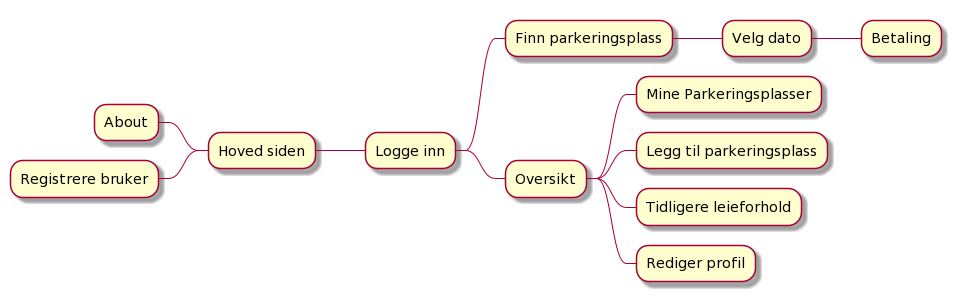
\includegraphics[width=12cm]{bilder/uml/oversikt.png}
    \caption{Oversikt over sidene i systemet}
    \label{fig:proto_overview}
\end{figure}
Figur \ref{fig:proto_overview} viser hvordan det er mulig å navigere rundt i systemet. Det meste av funksjonaliteten er lukket bak "Logge inn" siden for å begrense hva en hvilken som helst person kan se og hente ut av systemet. "About" og "Hovedsiden" inneholder ingen sensitiv informasjon og er tilgjengelig for alle for å gi en beskrivelse av hva systemet er. Deretter kan en bruker eventuelt velge å opprette en profil og få tilgang til systemet.

\subsubsection{Funksjonalitet og avgrensinger} 
\textbf{Tydelig hva slags krav som er dekket av prototypen }
Vi ønsker at prototypen skal vise det vi anser som den mest sentrale delen. Vi ønsker at den skal vise et MVP (Minimal viable product) hvor kunden kan få mest utbytte av prototypen tidligst mulig. Vi har sett på de ulike funksjonalitetene vi vil ha med, og kommet fram til ulike krav som er viktige i prototypen. Vår estimering utgjort i tabell \ref{tab:Kravestimering} har hjulpet oss med å se hva som bør prioriteres i prototypen og hva som kan tas med til senere utvikling. Våre User cases i seksjon \ref{user_case} har også bidratt til å avdekke den viktigste funksjonaliteten i systemet. Muligheten til å leie og legge ut en parkeringsplass er sentrale funksjoner som gir kunden mest utbytte og mulighet til å bruke prototypen, og dermed viktig å ha med i prototypen. Muligheten til å søke etter parkeringsplasser er også inkludert sammen med andre krav som gjør brukervennligheten av tjenesten bedre, slik at kunden kan få enda mer ut av prototypen. For vår prototype har vi valgt å fokusere på disse kravene:   

%Vi ønsker at prototypen skal vise det vi anser som den mest sentrale delen. Vi ønsker at den skal vise MBP hvor da kunden kan få mest utbytte av prototypen. Dermed har vi sett på de ulike funksjonalitetene vi vil ha med, og kommet til ulike krav som er viktige i prototypen. Som det å leie og legge ut en parkeringsplass er veldig viktige funksjoner som gir kunden mer utbytte og mulighet til å bruke prototypen. Vi har også valgt å inkludere krav som gjør brukervennligheten til kunden bedre, blant annet søk på parkeringsplasser.
For vår prototype har vi valgt å fokusere på disse kravene:
\begin{table}[H]
% \centering
\begin{tabular}{ll}
4.1.1.a & Opprette bruker m/ epost-adresse        \\
4.1.2.a & Logge inn m/ epost-adresse              \\
4.1.2.d & Feilmelding ved feil brukernavn/passord \\
4.1.3  & Legge inn parkeringsplass               \\
4.1.5  & Leie parkeringsplass                    \\
4.1.6  & Søk av parkeringsplass                  \\
4.1.7  & Brukerprofil                            \\
4.1.9  & Betaling                               
\end{tabular}
\end{table}
% \begin{itemize}
%     \item 4.1.1.a Opprette bruker m/ epost-adresse
%     \item 4.1.2.a Logge inn m/ epost-adresse
%     \item 4.1.2.d Feilmelding ved feil brukernavn/passord
%     \item 4.1.3 Legge inn parkeringsplass
%     \item 4.1.5 Leie parkeringsplass
%     \item 4.1.6 Søk av parkeringsplass
%     \item 4.1.7 Brukerprofil
%     \item 4.1.9 Betaling
% \end{itemize}
%\textit{* $\longrightarrow$ Her har vi fokusert på generelt for utleiere og ikke firma.} \\
%\textit{** $\longrightarrow$ Vi har valgt en lettere implementasjon, istedenfor kart er det poststed}\\
%\textit{*** $\longrightarrow$ Vi har valgt å vise oversikt over leide plasser og utleide plasser. Admin oversikt er ikke implementert, heller ikke oversikten vist med grafer.}\\
%\textit{**** $\longrightarrow$ Hoved kravet blir implementert, men ikke underkravene}
\vspace{-1em}
For hvert av disse kravene vil de mest viktigste delene bli implementert. Ergo de kravene som tidligst gir produkt til kunden. Det medfører at noen krav ikke blir implementert, blant annet administrator sine rolle i tjenesten og oversikten over inntjeninger i form av kakegraf.. 

 Brukere kan heller ikke se antall utilgjengelig og tilgjengelig plasser. Vi har implementert det slik at for en gitt adresse er det bare en parkeringsplass. Det medfører at Firma sin rolle ikke er implementert.


For krav om betaling er det hovedkravet som er i fokus. Det er da en demo av betalingsløsningen. Det medfører at betalingen er implementert med en enkel funksjon i vårt system som bestemmer om betalingen blir godkjent eller ikke. Dette kan bli implementert senere med de eksterne avhengighet som vi har valgt.
Det er også i fokus brukeren betaler for parkeringsplassen. Det medfører at firma ikke betaler for tjenesten eller at man ikke kan avbestille parkeringsplassen. Det kan bli implementert senere, og er ikke i fokus i vår prototype. Avbestilling også blir ikke prioritert, eller tjenesten sin konto. 


Søk av parkeringsplass er implementert i form av poststed. 


%Disse avgrensningene er listet under::
%\begin{enumerate}

%\item Systemet har kun en demo av en betalingsløsning. Det medfører at betalingen er implementert med en enkel løsning. Det er en enkel funksjon implementert i vårt system som bestemmer om betalingen blir godkjent eller ikke.

%\item Det er ikke implementert en avgiftsløsning for firmaer (prosentandel av salget) 

%\item Admin sin rollen er ikke implementert.

%\item Firma funksjonene er ikke implementert.
%\item Bruker kan ikke avbestille parkeringstjenesten.
%\item Søk av parkeringsplass har bare blitt implementert i form av poststed og ikke kart
%\end{enumerate}


\subsubsection{Modellering av prototypen}
\textbf{Diagrammer som beskriver relevatne deler av systemet eller prosessene (ikke nødvendigvis funksjoner i prototype). Elementene i diagrammene og funksjonaliteten deres er tydelig.}

Denne seksjonen vil vise modelleringen av prototypen og systemet. Det viser hvordan systemet/prototypens funksjoner samhandler. Det gjøres med forskjellige diagrammer som flytdiagram, aktivitetsdiagram, sekvensdiagram og lignende.
\paragraph{Opprette bruker modellering}
\begin{figure}[H]
    \centering
    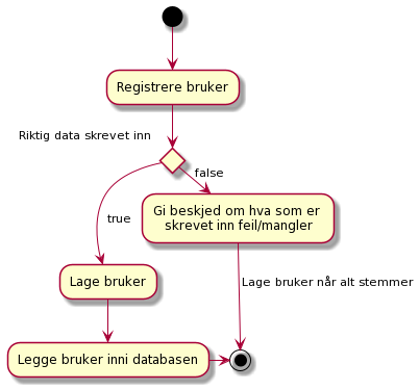
\includegraphics[width=5cm]{bilder/uml/registerebruke.png}
    \caption{Sekvensdiagram for opprette bruker}
    \label{fig:reg_bruker}
\end{figure}
Figur \ref{fig:reg_bruker} viser flyten i hvordan man registrerer en bruker. Dette kommer fra kravet 4.1.1.a hvor brukeren kan opprette en bruker med epost-adressen. Brukeren sender inn dataen sin via et skjema, systemet sjekker opp om dataen er skrevet inn riktig (om noe mangler, om det er riktig e-post og riktig telefonnummer), og hvis alt stemmer så blir profilen dannet og sendt videre til databasen. Hvis noe av informasjonen ikke er riktig så får brukeren beskjed om det slik at han kan rette det opp. 

Brukeren som blir registrert blir lagret i en json-fil istedenfor en database i vår prototype. Vi har gått for en litt mer lettvint løsning når det gjelder lagring av dataen, men siden fungerer fullstendig bortsett fra det.  

 
\paragraph{Logge inn modellering}

\begin{figure}[H]
\centering
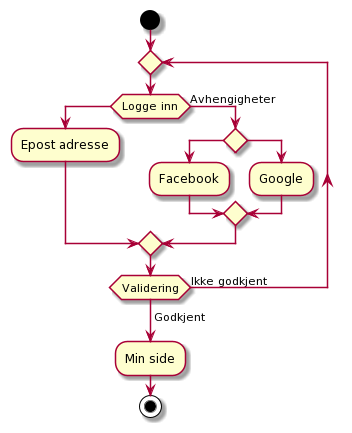
\includegraphics[width=5cm]{bilder/uml/loggeinn.png}
\caption{Aktivitetsdiagram for funksjonen å logge inn}
\label{fig:logginn}
\end{figure}
Figur \ref{fig:logginn} viser hvordan flyten skal være ved å logge inn. Dette kommer fra kravet 4.1.2 hvor da brukeren kan logge seg inn med enten Facebook, Google eller med epost-adresse. Figuren viser visuelt hvordan brukeren ser aktiviteten i kravet. Ved å logge inn blir det validert. Hvis det ikke blir godkjent blir man sendt til logge inn siden igjen. Hvis man får godkjent kommer man til Min side.

Facebook og Google er en ekstern avhengighet som vil da direkte komme til siden til facebook eller Google for å logge inn. I vår prototype er ikke dette implementert, da epost adresse innlogging gir verdi tidligst mulig for kunden. Dette er beskrevet i seksjonen om vår funksjonalitet og avgrensning av systemet.

\paragraph{Brukerprofil}
\begin{figure}[H]
    \centering
    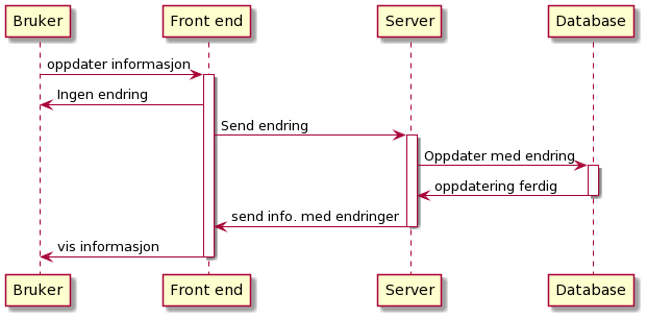
\includegraphics[width=10cm]{bilder/uml/brukerprofil.png}
    \caption{Sekvensdiagram for funksjonen endre informasjonen om brukeren lagret i vårt system }
    \label{fig:endre_bruker}
\end{figure}
Figur \ref{fig:endre_bruker} viser hvordan man gjør endring i brukerprofil. Skulle en bruker trykke på oppdater uten å ha gjort noen endringer kuttes prosessen av for å ikke gi unødvendig mye jobb for serveren. Videre sendes endringene til serverene som oppdaterer informasjonen i databasen. Når dette er gjort sendes den oppdaterte informasjonen tilbake til brukeren og vises i front end.

\paragraph{Søking av parkeringsplass}
\begin{figure}[H]
    \centering
    \includegraphics[width=5cm]{bilder/uml/søkeparkering.png}
    \caption{Aktivitetsdiagram for søking av parkeringsplass}
    \label{fig:search_parking}
\end{figure}
Figur \ref{fig:search_parking} viser hvordan brukeren oppfatter søking av parkeringplass fra krav 4.1.6 som omhandler å søke etter parkeringsplass. Det gir et visuelt bilde for brukeren hvordan søkingen går. De henter parkeringsplassene utifra poststedet eller lokasjonen i kartet. Disse hentes fra databasen.

I figuren ser du tydelig at man kan søke ved hjelp av kart. Dette gjør det lettere å finne nærmeste lokasjon. Det er også et ønske å sortere de etter visse egenskaper som for eksempel pris.

Vår prototype har fokusert på selve søkingen i form av poststed. 
\paragraph{Legge ut parkeringsplass}
\begin{figure}[H]
    \centering
    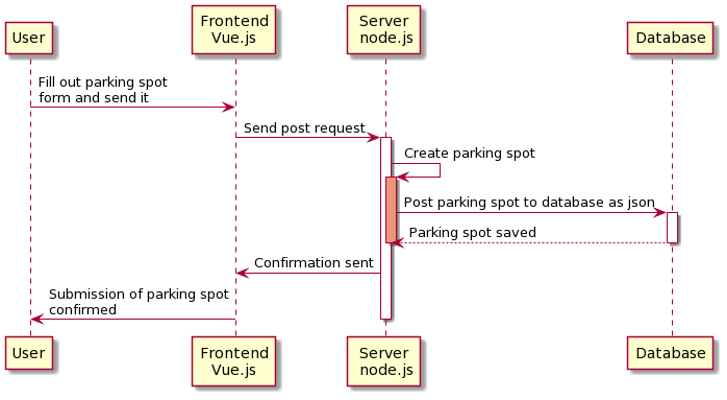
\includegraphics[width=10cm]{bilder/uml/legge_parkeringsplasss.png}
    \caption{Sekvensdiagram for legge ut parkeringsplass}
    \label{fig:legge}
\end{figure}
Figur \ref{fig:legge} viser til krav 4.1.4 som omhandler det å legge ut en parkeringsplass. Figuren viser at brukeren sender inn et skjema med data på nettsiden. Vue.js sender det videre til backend-en og oppretter en parkeringsplass. Parkeringsplassen blir sendt som json-data til databasen, og systemet sender en bekreftelse tilbake om at parkeringsplassen er lagt inn. På denne måten kan brukeren være sikker at alt ble gjennomført og parkeringsplassen er lagt inn siden det kommer en bekreftelse tilbake til brukeren som vist på figuren. 

Dette kravet er implementert fullstendig i vår prototype og fungerer som det skal. Vi har valgt å lagre dataen i en json-fil istedenfor en database for å gjøre løsninga mer lettvint.  
 
\paragraph{Betaling}
\begin{figure}[H]
    \centering
    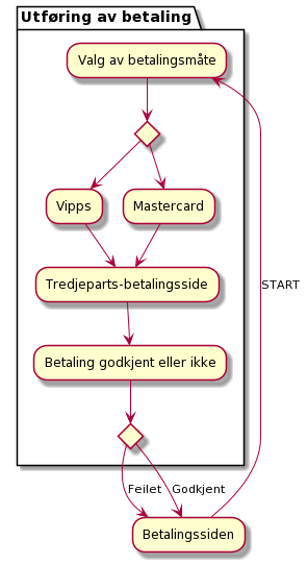
\includegraphics{bilder/uml/betaling.png}
    \caption{Flytdiagram for betalingen}
    \label{fig:betaling}
\end{figure}

En viktig del av systemet vil være betaling for tjenestene. Figur \ref{fig:betaling} viser hvordan betalingsdelen av systemet vil fungere. Dette kommer fra krav 4.1.8. Prototypen er en enkel versjon av systemet hvor betalingensdelen er avgrenset. En full versjon av betalingen vil kreve avtaler med Vipps og Mastercard.  

Først verifiseres det at «produktet» som skal bli kjøpt er tilgjengelig og at betalingsinformasjonen stemmer. Deretter velger kunden betalingsmåte og blir ført videre til den spesifikke betalingssiden. I prototypen blir det steget hoppet over og det vil bli gitt en direkte beskjed om godkjent eller feilet betaling. 




\subsubsection{Avhengigheter}
Noen av avhengighetene vi har er: 
\begin{enumerate}
    \item Javascript ES9 

    \item Vue.js 2.x

    \item BULMA som er et CSS rammeverk 

    \item Express rammeverk for å håndtere forespørsler 

    \item Versjon 14.13.0 av Node.js 

    \item  Jest rammeverk til testing 

    \item Pakkesystem npm som er en del av Node.js 
\end{enumerate}




\subsubsection{Kjente svakheter og problemer}
% \textit{Forklar ev. kjente svakheter og problemer med prototypen. Det er bedre at Kunden vet
% om problemer på forhånd før de ev. merker dem selv.}
% I og med at vårt produkt er en prototype, så er ikke alle kravene implementert, og heller er ikke systemet feilfritt. I vår prototype er det noen svakheter som
% \begin{enumerate}
%     \item Prototypen har ikke en database, slik at alt er lagret i minnet.
%     \item Man får ikke redigert plassen sin. 
%     \item De bookete datoene er ikke fjernet fra kalenderen.
%     \item Brukere kan booke parkeringsplass tidligere enn nå-tidspunktet samme dag.
%     \item Brukere kan bytte epost for å utvide gratisperioden ved bruk av systemet.
% \end{enumerate}

Prototypen er laget for å demonstrere noen av de sentrale funksjonene i tjenesten. Og er ikke ett ferdig utviklet produkt. Under utviklingen har vi kommet borti enkelte problemstillinger som vi enten ikke har løst på en skikkelig måte. Eller skal bli erstattet av andre komponenter i det ferdige produktet.

Prototypen har ikke en implementert en database. Vi ønsker at det ferdige produktet skal benyttes seg av en dokumentdatabase. For å simulere dette på enklest mulig måte har vi valg å skrive JSON-objekter til enkelt-filer på disk.

% Enkelte sider mangler. Vi har for eksempel ikke lagt ved siden som lar brukere rediger plassen sin. Funksjonalitet som lar bruker slette kontoen, eller plassen sin er heller ikke lagt til.

Nedtrekks meny til høyre i navigasjonen lukkes ikke etter at en ny side er trykket på. Dette er en konflikt mellom BULMA og Vue.

For at dato velgeren skulle fungere på en god måte valgte vi å bruke v-calendar. Denne så lovende ut og var godt dokumentert. Men det lå noen problemer i den med vårt tenkte formål. Den lar oss ikke hente datoer fra databasen og legge disse til som utilgjengelige. Dette medfører at flere brukere kan reservere samme dag. Ved å bruke vue sin v-model funksjon på utilgjengelige datoer ender vi opp med å skape en konflikt med kalender komponenten.
Når man velger dagens dato kan man reservere plassen fra ett tidligere klokkeslett enn det som er nå.

Ved å være inne på betaling, eller velg dato sidene, og oppdatere siden. Vil systemet miste den plassen man holder på å reservere. Det er ikke laget noe funksjonalitet som skal håndtere denne feilen.

APIen kontrollerer ikke om dataen som bli sendt fra brukergrensesnittet faktisk er riktig. Det er kun lagt til «requierd» egenskaper på html elementene. Men dette kan endres i DOM, og dermed kan systemet enkelt bli utnyttet.


\subsection{Eksempler}
For å vise hvordan en bruker vil benytte seg av systemet så har vi hentet ut noen eksempler fra prototypen.

\subsubsection{Profilside}
Etter at en bruker har logget inn vil de komme til sin profil-side. Her får de en oversikt over sine plasser, og tidligere leieforhold.

\begin{figure}[H]
    \centering
    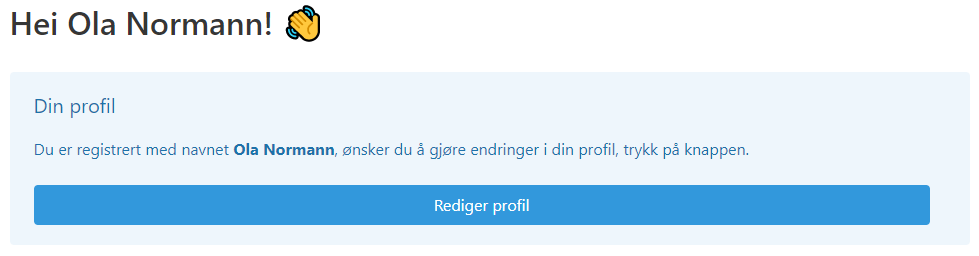
\includegraphics[width=10cm]{bilder/Eksempler/profile_start.png}
    \caption{Passende tekst}
    \label{fig:eks:profile}
\end{figure}

På toppen av siden vil brukeren får mulighet til å få videre for å redigere sine kontoopplysninger.

\begin{figure}[H]
    \centering
    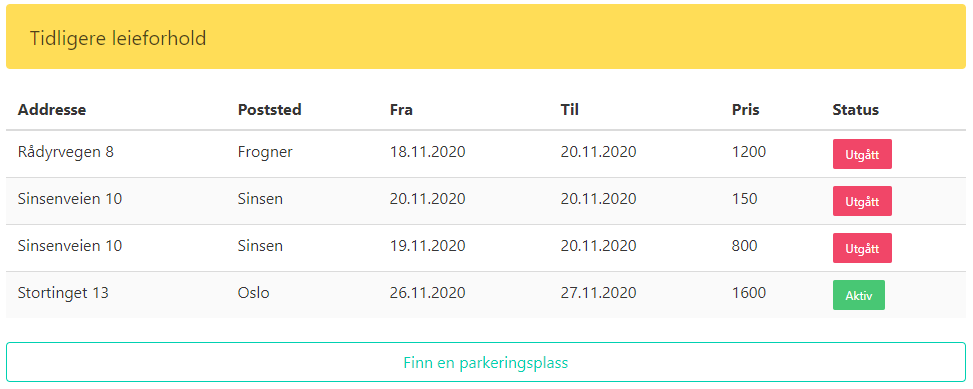
\includegraphics[width=10cm]{bilder/Eksempler/tidligere_leide_plasser.png}
    \caption{Passende tekst}
    \label{fig:eks:profile_leide}
\end{figure}

Det vil bli vist en oversikt over deres tidligere leieforhold. Med en status om parkeringen fortsatt er gyldig eller har utgått.

\begin{figure}[H]
    \centering
    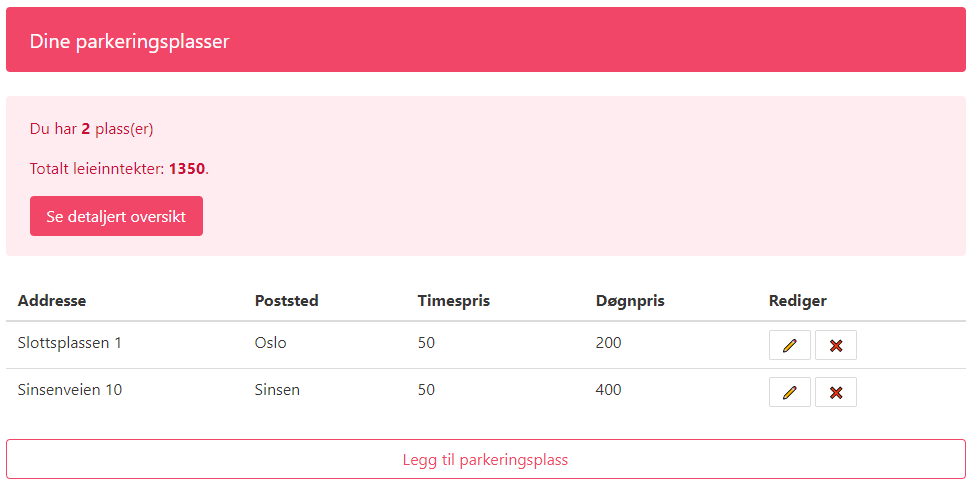
\includegraphics[width=10cm]{bilder/Eksempler/dine_plasser.png}
    \caption{Passende tekst}
    \label{fig:eks:profile_spots}
\end{figure}

Nederst vil de får oversikt over parkeringsplasser de selv leier ut. Og med en samlet inntjening av plassene sine.

\subsubsection{Leie parkeringsplass}
For å leie en plass, trykkes det på knappen «Finn parkeringsplass», som vil ta dem til siden hvor man får en oversikt over tilgjengelige plasser.

\begin{figure}[H]
    \centering
    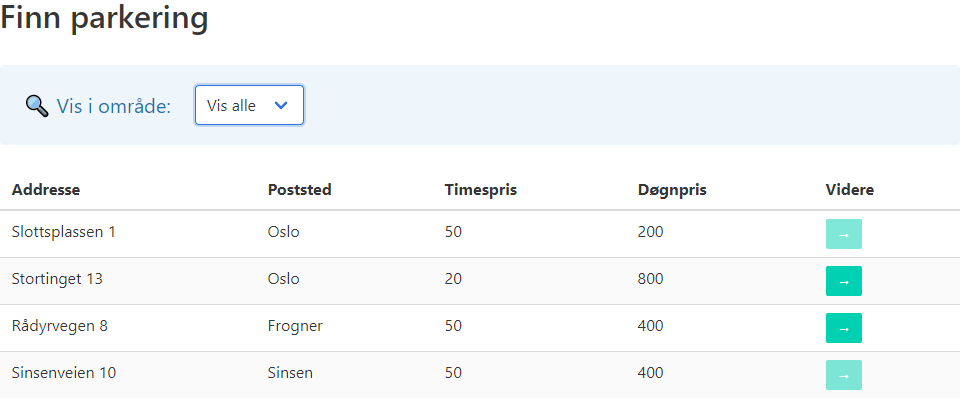
\includegraphics[width=10cm]{bilder/Eksempler/finnparkering.png}
    \caption{Passende tekst}
    \label{fig:eks:findspots}
\end{figure}

Det aktuelle området man leter etter plass kan filtreres ved å bruke nedtrekks menyen. Plasser merket med lysegrønn videre-knapp er brukeren sine egne plasser. Og kan ikke velges.

\begin{figure}[H]
    \centering
    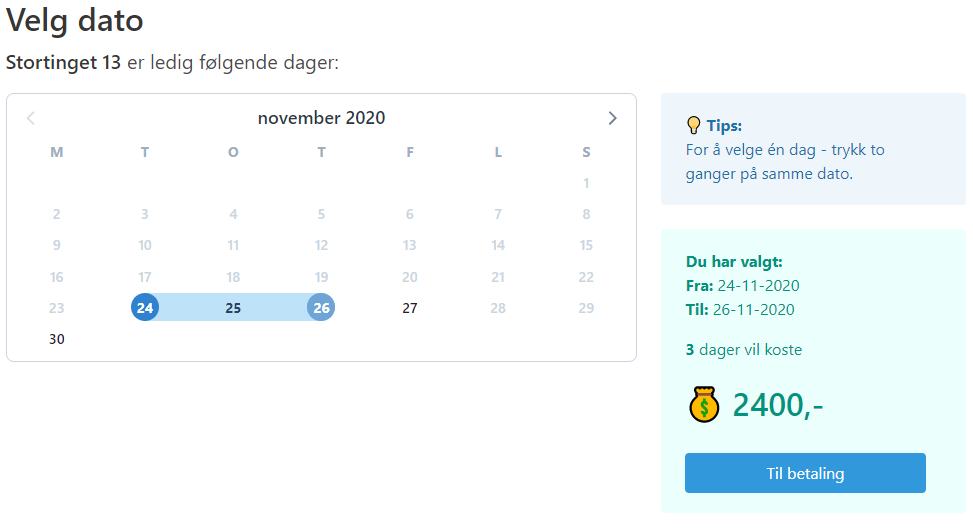
\includegraphics[width=10cm]{bilder/Eksempler/velgdato_dager.png}
    \caption{Passende tekst}
    \label{fig:eks:findspots_days}
\end{figure}

Når brukeren har funnet ønsket plass, velger man tilgjengelig dato i kalenderen. For å leie plass i flere dager velger man til og fra dato. Estimert kostnad for perioden vil bli vist på høyre side.

\begin{figure}[H]
    \centering
    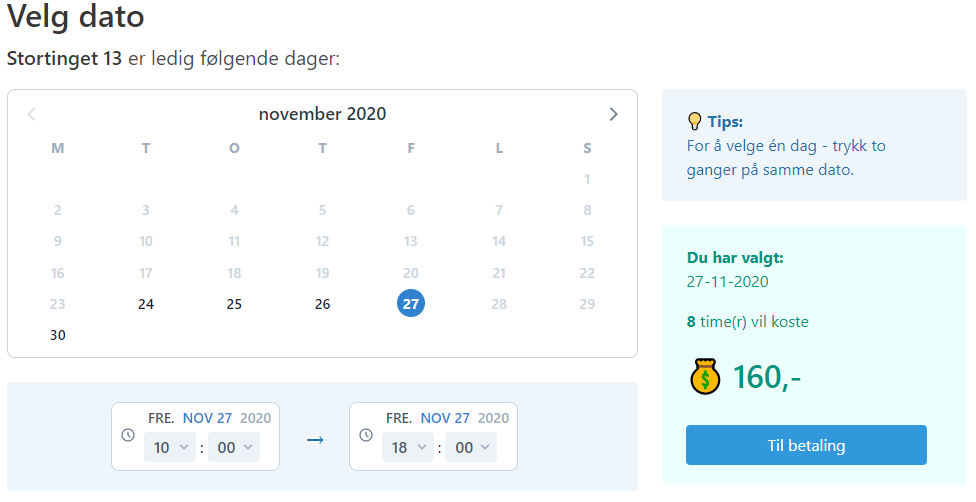
\includegraphics[width=10cm]{bilder/Eksempler/velgdato_timer.png}
    \caption{Passende tekst}
    \label{fig:eks:findspots_hour}
\end{figure}

Hvis det er ønskelig å leie plass kun for noen timer velger man én dato. Det vil da være mulig å spesifisere fra og til klokkeslett de ønsker å leie plassen. Estimert kostnad for perioden vil bli vist på høyre side.

Ved å trykke på «Til betaling» går man videre til betalingssiden.

\begin{figure}[H]
    \centering
    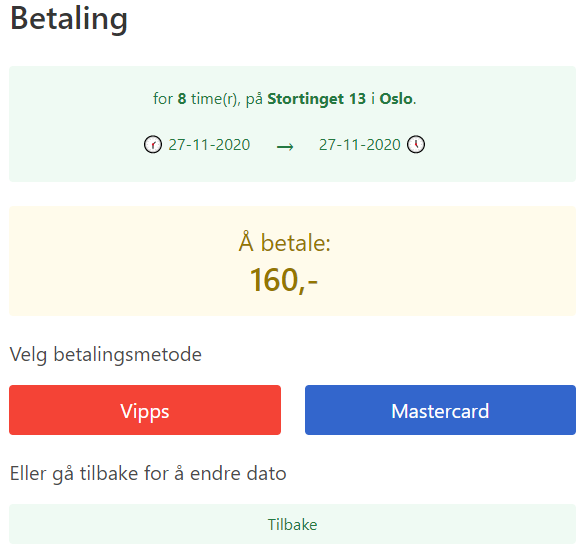
\includegraphics[width=7cm]{bilder/Eksempler/betaling.png}
    \caption{Passende tekst}
    \label{fig:eks:findspots_pay}
\end{figure}

Her blir man vist en oppsummering av bestillingen, og mulighet for å velge betalingsmåte.

\subsection{Installasjon av systemet}
For å installere og bruke systemet kreves Node og en nettleser. Vi har under utvikling brukt \href{https://www.google.com/intl/no/chrome/}{Google Chrome}, og Node versjon v14.13.0. Systemet har også blitt testet og virker med seneste versjon v15.2.1. For å installere Node se fremgangsmåte på deres \href{https://nodejs.org/en/}{hjemmeside}.

Vedlagt produktdokumentasjonen ligger en mappe: «Software-Engineering» som inneholder kildekoden til prototypen. For å fortsette installasjonen av nødvendige avhengigheter trenger vi å åpne terminalen og naviger inn i mappen.

\begin{minted}
[
frame=single,
framesep=10pt,
fontsize=\scriptsize,
breaklines
]
{bash}
$ cd Software-Engineering
\end{minted}

\subsubsection{Server}
Systemet er delt opp i to deler, en \textit{client} og en \textit{server}. Vi skal nå gå igjennom installasjonen av serveren.

I terminalen, naviger inn i \textit{server} mappen, og installer avhengigheter:

\begin{minted}
[
frame=single,
framesep=10pt,
fontsize=\scriptsize,
breaklines
]
{bash}
$ cd server
$ npm install
\end{minted}

\texttt{npm} vill nå laste ned alle avhengigheter til server programmet, og legge disse i mappen \textit{node\_modules}.

Når avhengigheten er ferdig lastet ned er server siden av systemet klart til bruk.

\subsubsection{Client}
Naviger terminalen inn i \textit{client} mappen og installer avhengigheter:

\begin{minted}
[
frame=single,
framesep=10pt,
fontsize=\scriptsize,
breaklines
]
{bash}
$ cd ..\client\
$ npm install
\end{minted}

\texttt{npm} vill nå laste ned alle avhengigheter til klient programmet, og legge disse i mappen \textit{node\_modules}.

Når avhengigheten er ferdig lastet ned er klient siden av systemet klart til bruk.

\subsection{Bruk}
Når avhengigheter til server og klienten er lastet ned og installert er systemet kart til bruk.
\textbf{Merk:} Både \textit{server} og \textit{client} må kjøre for at systemet skal virke som det skal!

\subsubsection{Server}
Vi åpner en ny terminal og navigerer først til \textit{server} mappen. Og starter serveren ved å bruke kommandoen:

\begin{minted}
[
frame=single,
framesep=10pt,
fontsize=\scriptsize,
breaklines
]
{bash}
$ npm run start
\end{minted}

Du vil nå få en tilbakemelding i terminalen som ser slik ut, systemet er klart til bruk på \href{http://localhost:5000}{http://localhost:5000}. Ikke lukk dette terminalvinduet for da avsluttes programmet.

\begin{minted}
[
frame=single,
framesep=10pt,
fontsize=\scriptsize,
breaklines
]
{bash}
> share-a-spot@1.0.0 start
> node index.js

Server running on port: http://localhost:5000
\end{minted}

\textbf{MERK!} Pass på at det ikke er noe annet på maskinen din som allerede kjører på denne porten, dette vill medføre at systemet ikke starter!

Hvis du åpner \href{http://localhost:5000}{http://localhost:5000} i nettleseren din, så skal du se meldingen:
\begin{minted}
[
frame=single,
framesep=10pt,
fontsize=\scriptsize,
breaklines
]
{bash}
{
  message: "Share-A-Spot Server - Up and running"
}
\end{minted}

\subsubsection{Client}
For å starte brukergrensesnittet, åpner vi ett nytt terminalvindu og navigerer til \textit{client} mappen. Vi starter vue sitt utviklingsmiljø ved:
\begin{minted}
[
frame=single,
framesep=10pt,
fontsize=\scriptsize,
breaklines
]
{bash}
$ npm run serve
\end{minted}

Dette vil bygge systemet og gjøre det klart til bruk.
\begin{minted}
[
frame=single,
framesep=10pt,
fontsize=\scriptsize,
breaklines
]
{bash}
App running at:
- Local:   http://localhost:8080/
- Network: http://192.168.1.XXX:8080/

Note that the development build is not optimized.
To create a production build, run npm run build.
\end{minted}

Når det er ferdig vil vi få en tilbakemleding i terminalen at systemet er tilgjengelig på \href{http://localhost:8080}{http://localhost:8080}. Ikke lukk dette terminalvinduet for da avsluttes programmet.

Når begge tjenestene kjører, er systemet klart til å brukes. Du kan nå åpne nettleseren din og navigere til \href{http://localhost:8080}{http://localhost:8080} hvor brukergrensesnittet er.

\subsection{Testing}
Systemet består av et brukergrensesnitt og en API som håndterer forretningslogikk. Det er mot APIen vi har fokusert på å skrive testene. Dette i all hovedsak for at brukergrensesnittet kun viser data som er sendt fra APIen, og det er skal være minimalt med logikk som ligger her.

Vi har skrevet tester mot alle funksjonene i APIen, men ut ifra kildekode oversikten, så er det ett par spesielle punkter hvor vi ikke har gjenskapt enkelte feil-tilfeller. Dette gjelder spesielle tilfeller i noen av funksjonene våre, hvor vi sender en feilmelding tilbake hvis databasen ikke klarer å skrive. Dette scenarioet har vi ikke skrevet en test for. Men logikken for å håndtere det er der. 

En annen test som ikke er fullstendig, er betalingen. Her er det skrevet kode som gjør at betalingen feiler cirka 20\% av gangene. Vi fant ingen løsning for å teste denne funksjonen på en god måte, så det vi gjorde er i stedet var å forvente at systemet ikke feiler, altså ikke gi «500 Internal Server Error». 

\subsubsection{Oversikt over filer}
Testene som tilhører funksjoner forbundet med innlogging finnes i filen \\ \texttt{login.test.js}.

\begin{table}[H]
\centering
\begin{tabularx}{\textwidth}{r|X}
% \begin{tabular}{@{}ll@{}}
4.1.2.a & Logge inn m/ epost-adresse              \\ 
4.1.2.d & Feilmelding ved feil brukernavn/passord \\ 
% \end{tabular}
\end{tabularx}
\end{table}



Brukere skal kunne opprette en konto i tjenesten, og ha en form for brukerprofil med noe funksjonalitet. Tester til følgende krav og funksjoner finnes i filen \texttt{user.test.js}

\begin{table}[H]
\centering
\begin{tabularx}{\textwidth}{r|X}
% \begin{tabular}{@{}ll@{}}
4.1.1.a & Opprette   bruker m/ epost-adresse \\
\ref{bruker_profil}  & Brukerprofil                       \\
% \end{tabular}
\end{tabularx}
\end{table}

Tester til funksjoner relatert til krav om å legge inn og leie plass finnes i filen \texttt{spots.test.js}



\begin{table}[H]
\centering
\begin{tabularx}{\textwidth}{r|X}
% \begin{tabular}{@{}ll@{}}
\ref{Legge_parkering} & Legge inn   parkeringsplass \\ 
\ref{leie_park} & Leie   parkeringsplass      \\
\ref{søke_park} & Søk av   parkeringsplass    \\
\ref{betaling} & Betaling                    \\ 
% \end{tabular}
\end{tabularx}
\end{table}

\subsubsection{Kjøre tester}
For å kjøre testene åpner vi en terminal og navigerer til \texttt{server} mappen. Vi bruker \href{https://jestjs.io/}{Jest} som er ett test rammeverk for JavaScript. Den vil gå igjennom alle mappene å lete etter filer merket med \texttt{<filnavn>.test.js}. Alle filer som ligger i mappen \texttt{\_\_tests\_\_} vil automatisk også bli kjørt. Alle testene til programmet vårt ligger i denne mappen.

Når vi er i \texttt{server} mappen starter vi testene ved:
\begin{minted}
[
frame=single,
framesep=10pt,
fontsize=\scriptsize,
breaklines
]
{bash}
$ npm run test
\end{minted}

Dette vil kun gi oss en tilbakemelding at alle testene var vellykket, eller hvis noen har feilet så vil den gi en tilbakemelding om det. For en mer utdypende rapport bruker vi \texttt{--verbose}. Merk, vi trenger \texttt{--} før \texttt{--verbose}.

\begin{minted}
[
frame=single,
framesep=10pt,
fontsize=\scriptsize,
breaklines
]
{bash}
$ npm run test -- --verbose
\end{minted}

Her får vi nå en oversikt over alle testene som blir kjørt med navnende deres. Disse navnene er også beskrivende slik at det er tydelig hva de tester. Se utdrag fra eksempel:

\begin{minted}
[
frame=single,
framesep=10pt,
fontsize=\scriptsize,
breaklines
]
{bash}
 PASS  __tests__/login.test.js
  GET / *
    OK / - Should respond with 403 - Forbidden (56 ms)
    OK / * (any) - Should respond with 403 - Forbidden (6 ms)
  POST /login
    OK Valid username and password should respond 200 (28 ms)
    OK Invalid username and password should respond 400 (6 ms)
\end{minted}

For få se hvor mye av koden testene faktisk dekker kan vi bruke en annen kommando \texttt{--coverage}.

\begin{minted}
[
frame=single,
framesep=10pt,
fontsize=\scriptsize,
breaklines
]
{bash}
$ npm run test -- --coverage
\end{minted}

Dette vil skape en oversiktlig rapport over hvilke filer som blir testet, hvor mye av koden i filene som blir dekket. Og hvis det er noen deler av koden vi ikke har inkludert. I tillegg lager jest en flott rapport som kan åpnes i nettleseren. Her kan man gå inn i de forskjellige filene, og detaljert se koden, og hvor testene eventuelt ikke dekker. Denne rapporten finner man under \texttt{coverage/Icov-report/index.html}.

\end{document}
